\documentclass[a4paper,12pt]{article}
\usepackage{graphicx}
\usepackage{amsmath, amsfonts}
\usepackage{amssymb}

\usepackage[utf8x]{inputenc}
\usepackage[T1]{fontenc}

\usepackage{lmodern}
\usepackage{textcomp}

\usepackage[round]{natbib}
%\usepackage{biblatex}
%\addbibresource{references.bib}

% \usepackage{babel}

% \usepackage{titlesec}

\usepackage[top=1.2in,bottom=1.2in,left=3.cm,right=3.cm,a4paper]{geometry}

\usepackage[font=footnotesize]{caption}

\usepackage{xcolor}

\usepackage{hyperref}

\usepackage{gensymb}
\hypersetup{
    colorlinks,
    linkcolor={red!50!black},
    citecolor={blue!50!black},
    urlcolor={blue!99!black}
}

\usepackage{titling}

%\interfootnotelinepenalty=10000

\pretitle{%

\includegraphics[width=0.3\linewidth]{fig/logo_UGA}
\vspace{2cm}
\begin{center}
\LARGE
}
\posttitle{\end{center}
\vspace{1cm}
}
\postdate{\par\end{center}\vspace{12cm}~}

\usepackage[nottoc,numbib]{tocbibind}
\usepackage{footnote}
\makesavenoteenv{tabular}
\makesavenoteenv{table}
%%%%%%%%%%%%%%%%%%%%%%%%%%%%%%%%%%%%%%%%%%%%%%%%%%%%%%%%
\title{Measurements of Turbulence in Katabatic Wind}
\author{Claudio Pierard \\
\\
\\
Master 1 Applied Mechanics\\
\\
Supervisor: Jean-Emmanuel Sicart}

% to define new commands
\newcommand{\R}{\mathcal{R}}
\newcommand{\mean}[1]{\langle #1 \rangle}

% to show the pieces of advice
\newcommand{\advice}[1]{{\it #1}}
% to hide the pieces of advice
% \newcommand{\advice}[1]{}

\begin{document}

\renewcommand{\labelitemi}{$\bullet$}

\maketitle
\begin{abstract}
The study of katabatic winds is relevant because it influences the weather and pollution condition of the valleys in mountainous regions. We propose a field case study of the katabatic winds in the Belledonne Massif, with the objective of measuring the turbulence of the downslope jet and characterise it. We present the basic concepts necessary to study the katabatic winds and the objectives for the proposed project based on previous studies done by students that worked on it before. In the end, a work plan or schedule is presented which describes the activities to do during the next months.
   
\end{abstract}

\newpage

\tableofcontents

\newpage

\section{Introduction}

Katabatic winds or gravity currents are downslope winds that are generated when cold dense air is accelerated down a topographic slope due to surface cooling that gives the air a greater density than the free atmosphere~\citep{poulos2008observational}. They can be found in many places over the world, but they are mostly present in mountainous regions.

Katabatic winds play an important role in the local weather and the dispersion of contaminants in the valleys. These winds can flow down the mountains and fill the cool air pools that accumulate in the valleys. This can result in temperature inversions, which have negative effects on urban valleys where pollution is present~\citep{largeron2016persistent}. Nowadays, katabatic winds are not well represented or parameterised in the mesoscale models for weather forecast and this can cause errors in the forecasts for mountainous regions. There have been several studies of katabatic winds historically, mostly centred in the alpine regions of Europe, some parts of North America, Greenland and Antarctica. Despite this, there is a lack of suitable data obtained from measurements that can be used to test or adapt the theoretical models of katabatic winds~\citep{manins1979katabatic}. This is why is relevant a field case study of these winds.

\section{Theory}

In this section we introduce and define some of the concepts necessary for this project, starting from the boundary layer structure to the specifics of the turbulent quantities necessary for its characterisation.

\subsection{Boundary layer structure}
The planetary boundary layer or atmospheric boundary layer (ABL) is defined as the part of the troposphere that is in contact with the surface and that is directly influenced by surface forcings, such as friction, evaporation, heat transfer, emission of contaminants and by the soil~\citep{stull2012introduction}. The thickness or height of the ABL varies throughout the day and depends on the location. Mainly the height varies by the incidence of solar radiation on the surface, which makes the air parcels in contact with the surface acquire more flotation, generating convection.

\begin{figure}[ht!]
	\vspace{-5pt}
    \centering
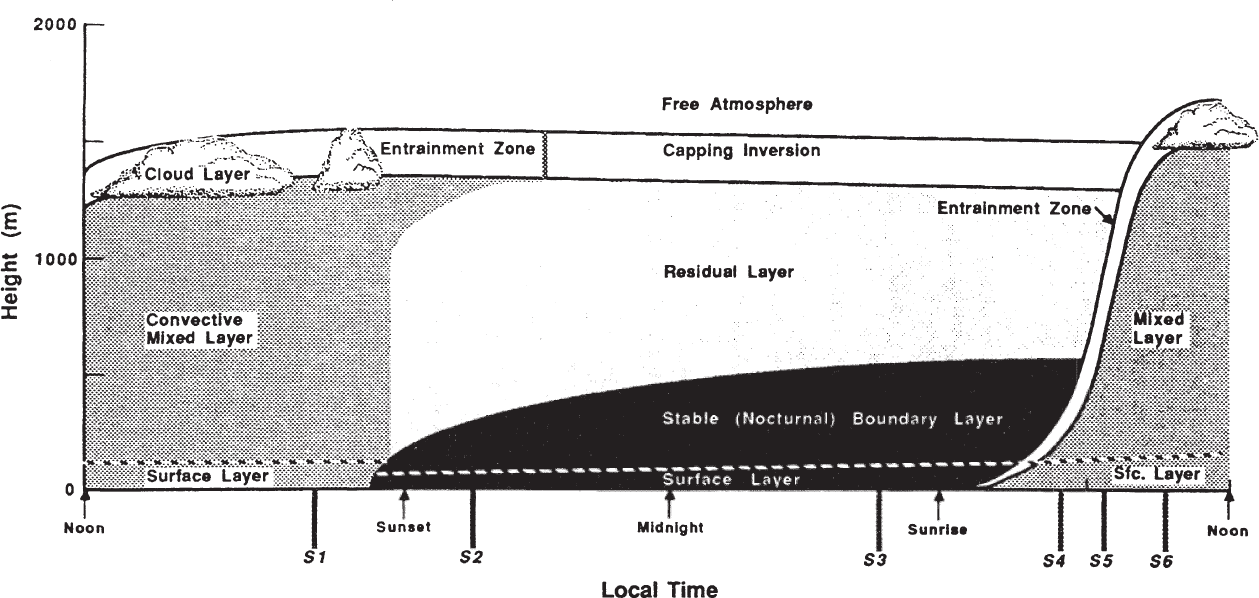
\includegraphics[width=0.9\textwidth]{fig/abl_stull.png}
    \caption{Diagram of the daily evolution of the structure of the ABL. Image based on the boundary layer scheme of \cite{stull2012introduction}.}
    \label{fig:ABL_structure}
  \vspace{-5pt}
\end{figure}

The figure~\ref{fig:ABL_structure} shows the structure and temporal evolution of the ABL, its components are the mixing layer, the residual layer and the stable boundary layer. Each of these has special characteristics and different physical processes that distinguish them. To understand the dynamics of the planetary boundary layer it is necessary to define each of them. However, in this study, we focus mostly on the stable nocturnal boundary layer, because is during the occurrence of this layer that katabatic winds form~\citep{poulos2008observational, stull2012introduction}.

\subsubsection{Stable boundary layer}
The stable nocturnal boundary layer is formed during the night when the sunlight stops reaching the ground. This layer is characterised by sporadic turbulence caused by wind shear and the contact with the surface, with a tendency to suppress turbulence. The upper limit of the stable boundary layer is located at the height where the intensity of the turbulence is a small fraction of its surface value. The air in this layer is statically stable, opposed as its daytime equivalent, the mixed layer~\citep{stull2012introduction}.

When the stable boundary layer is formed, the air that is close to the ground cools down and can form drainage winds or katabatic winds, only if there is a slope in the topography.

\subsection{Katabatic wind}

The katabatic winds are local winds that are created in presence of a descending terrain gradient when air masses flow downslope, continuously being cooled by radiative processes near the ground. They are a ventilation mechanism in mountainous regions~\citep{manins1979model}. Normally, these winds are shallow, where the thickness of the jet can go from 2 to 20~m. They have velocities on the order of 1 to 5~m/s \citep{stull2012introduction}. 

\begin{figure}[ht!]
	\vspace{-5pt}
    \centering
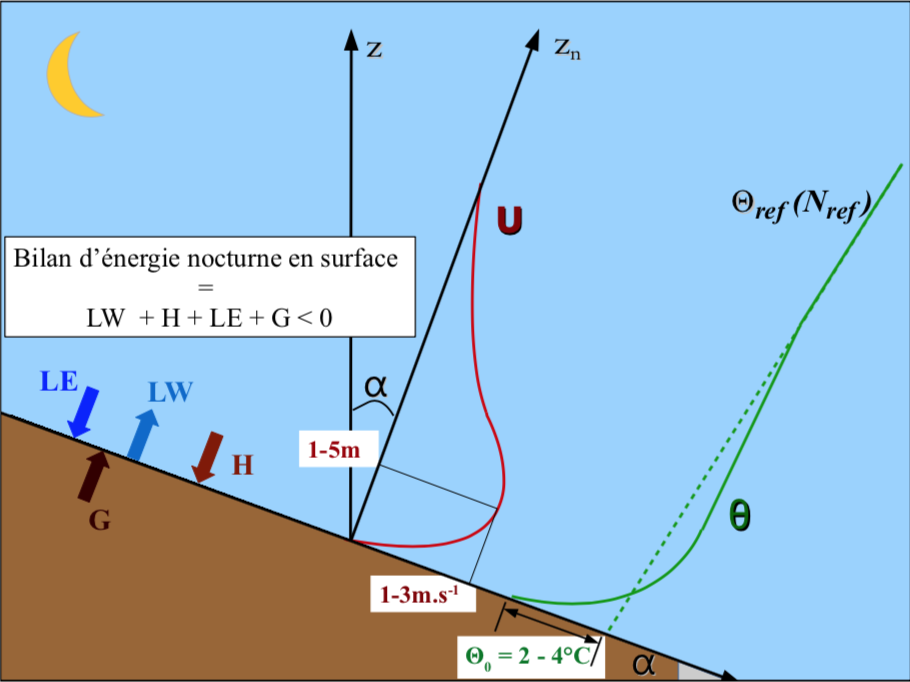
\includegraphics[width=0.6\textwidth]{fig/profiles_katabatic_wind.png}
    \caption{Characteristic wind profile (red) and potential profile (green) of the katabatic wind. Image from~\cite{claudine}.}
    \label{fig:u_profile}
  \vspace{-5pt}
\end{figure}

These winds are characterised for having a velocity profile as the one shown in the red curve in figure~\ref{fig:u_profile}. We can see that near the surface the velocity grows as we go up until it reaches a maximum and starts to decrease. This is the theoretical velocity profile of the katabatic winds. Also in figure~\ref{fig:u_profile}, we can see in the green curve the profile for the potential temperature, where we the theoretical profile shows that it grows rapidly as we go up until a point were it remains constant. This theoretical results can be useful to detect the occurrence of katabatic wind in the data sets.

An important factor to highlight about the katabatic winds is that external factors like synoptic or mesoscale winds can alter or destroy this kind of local winds~\citep{stull2012introduction}. The katabatic winds are important under conditions of slack synoptic pressure gradients~\citep{manins1979katabatic}. This factor plays an important role in the planning out the field campaign because we want to measure the katabatic jet as undisturbed as possible. For this, we are looking for a meteorological window when anticyclonic conditions will be present. 

\subsection{Turbulence Kinetic Energy (TKE)}
Commonly the TKE is defined as the kinetic energy per unit mass. This is one of the most important quantities to characterise turbulence in a flow, by giving us information about whether a region will become more turbulent, or whether turbulence will decay~\citep{stull2012introduction}.  Is defined as:

\begin{equation}
    e = \frac{1}{2} \big(\bar{u}^2 + \bar{v}^2 + \bar{w}^2\big). 
    \label{eq:tke}
\end{equation}

 Using the Reynolds averaging method for the velocity components
\begin{equation}
   u_i = U_i + u'_i,
   \label{eq:Re_avg}
\end{equation}


\noindent where $U_i$ is the average speed in one component and $u'_i$ is the fluctuations around the average. Substituting the previous equation in~\ref{eq:tke} and doing some simplification we get

\begin{subequations}
  \begin{align}
    e &= \frac{1}{2} \big((\overline{U + u'})^2 + (\overline{V + v'})^2 + (\overline{W + w'})^2 \big), \\
    &= \frac{1}{2} \big(\overline{u'^2} + \overline{v'^2} + \overline{w'^2}\big),
  \end{align}
  \label{eq:tke_2}
\end{subequations}

\noindent which is the definition of turbulent kinetic energy (TKE). The over-line represents the average of the variable. 

\subsection{Covariance}

Recalling the classical definition of covariance between to variables, we have the relation 

\begin{equation}
    \text{covar}(A,B) = \frac{1}{N}\sum_{i=0}^{N-1} (A_i - \overline{A})(B_i - \overline{B}).
\end{equation}

\noindent Using the Reynolds averaging method in the previous expression we get:

\begin{subequations}
\begin{align}
    \text{covar}(A,B) &= \frac{1}{N}\sum_{i=0}^{N-1} a_i' b_i', \\
    &= \overline{a'b'}.
\end{align}
\end{subequations}

\noindent This is the mathematical definition of covariance for a turbulent flow. The covariance indicates the degree of common relationship between two variables~\citep{stull2012introduction}. Is the principle by which we define the eddy fluxes.

\subsection{Eddy Flux}
According to \cite{stull2012introduction}, a turbulent flux or eddy flux is the transport of a physical quantity by the effect of the turbulence. In this project, we are mostly concerned with the sensible heat flux and the momentum flux in the katabatic jet. The sensible heat flux is given by the expression:

\begin{equation}
    H = \rho \ C_p \ \overline{w'\theta'},
\end{equation}

\noindent where $C_p$ is the specific heat at constant pressure and $\theta '$ is the fluctuations in potential temperature. We are interested in the vertical flux of the sensible heat, that is why we use the vertical wind fluctuation $w'$.

The momentum flux is given by the expression

\begin{equation}
    F = \rho \ \overline{u'w'}, 
\end{equation}

\noindent where $\rho$ is the density of air, and $u'$ and $w'$ are the fluctuations of velocity in the x-coordinate and in the vertical coordinate. The latter expression also is known as a component of the \textbf{Reynolds stress tensor}. The Reynolds stress describes all the components of the momentum flux in a control volume.

\section{Methodology}
My project is based on the work done by previous students, who made their master thesis on the same subject but with different data sets obtained from previous field campaigns. In Particular, \cite{jakob} processed the data of the 2015 campaign, that took place from 7 to 22 April 2015, during an episode anticyclonic conditions. In his work, he had to detect the days in which the instruments measured katabatic winds. For this, he used the past records of the meteorological report to see when there were anticyclonic weather conditions. Also, he analysed the wind profiles and temperature profiles to see if they fitted the description of the katabatic winds. After selecting the days, he computed the Reynolds stress tensor, the sensible heat flux and the turbulent kinetic energy. Is important to highlight that he analysed the region where the maximum of the velocity of the jet is expected to be. As a suggestion for future projects, he points out that it could be interesting to study the turbulence beneath the wind maximum, by placing more sensors in the lower levels of the masts (see section~\ref{instrumentation}).

Also, my work takes in to account the previous work done by \cite{claudine} and \cite{alban}. Both of them analysed the data from the November 2012 campaign. They followed the same methodology as \citeauthor{jakob} did, analysing the same turbulence characteristics of the jet. The main difference is that their work is focused on adapting the Prandtl analytical model with the different measurements recorded in the field. Another difference is that \citeauthor{claudine} did a spectral analysis of the data. This allowed her to represent the energy as a function of the frequency, with the objective to see the energy cascade characteristic of turbulence. 

\subsection{Objectives}
My objectives for this research project will be to analyse the data from a new mission planned for this the months of January or February, in which there are more sensors installed especially in the bottom and the lower region of the meteorological stations (see section~\ref{instrumentation}). This tackles the limitations found in the previous works mentioned above. 

More specifically, the first step will be to pre-process the data using the EddyPro Software (eddy covariance method). Then, it will be necessary to detect the katabatic wind episodes in the data set, by selecting the data that coincide with the anticyclonic episodes and which temperature and wind profiles coincide with the description of the katabatic winds. After that, I will analyse all the turbulent characteristics of the turbulent jet as \citeauthor{jakob} did. And finally, I will do the spectral analysis of the data as \citeauthor{claudine} did. 

There exist the possibility that the meteorological conditions necessary to do the measurements won't occur during winter or occur after February. In this case, I will analyse the data of 2015 and complete the analyse already done by \citeauthor{jakob}, by doing a spectral analysis of the signals, as \citeauthor{claudine} did with the 2012 data sets.

\subsection{Observational site}

The field campaign is planned to be held in the west face of the Grand Colon mountain, in Belledonne Massif, 10~km at the southeast of Grenoble. A topographic map of the area is shown in figure~\ref{fig:obs_site}, where the measuring site is marked with a red cross.

\begin{figure}[!ht]
  \begin{center}
  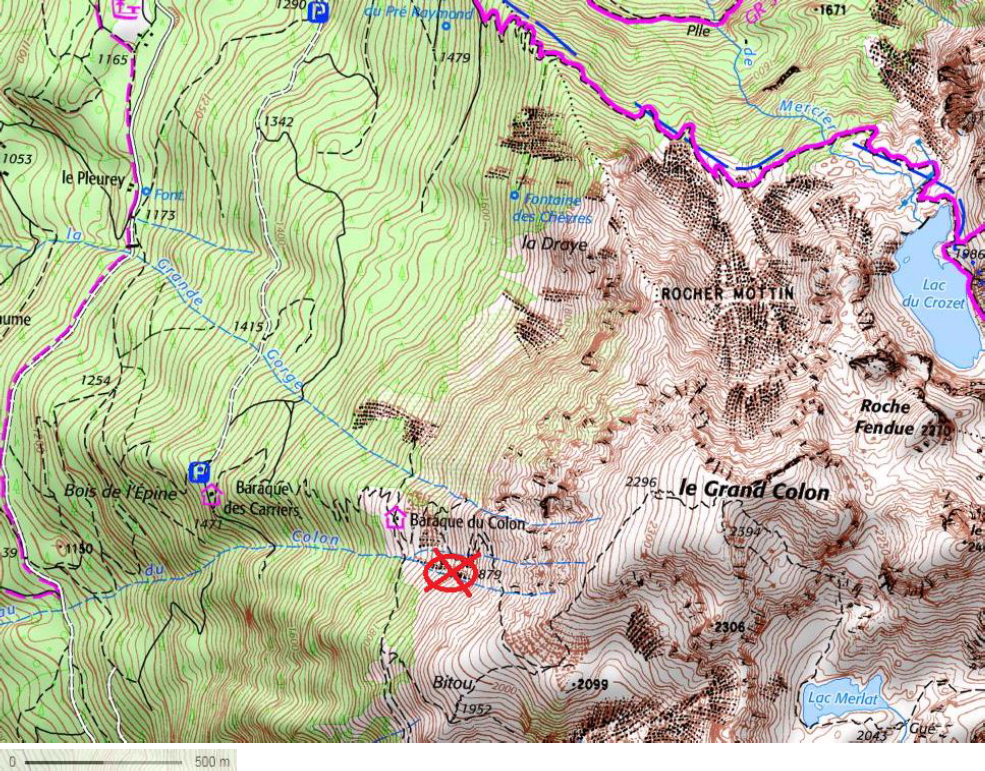
\includegraphics[width=0.8\textwidth]{fig/grand_colon_jakob.png}
  \caption{Topographic map of the Grand Colon. The red cross marks the location of the measuring site. Map from~\cite{jakob}.}
  \label{fig:obs_site}
  \end{center}
\end{figure}

The slope in the observational site is $21\degree$. The meteorological station is going to be located at an altitude of 1770 metres above sea level~\citep{claudine}. All the characterisation of the topography has been done by \cite{alban}.

\subsection{Instrumentation} \label{instrumentation}
The instruments for the next field campaign will be assembled into two masts, which will be located side by side. The mast has been reconfigured to tackle some of the problems and limitations from previous campaigns. We distinguish them by their height, one is 6~m high and the other is 12~m high\footnote{The configuration was altered recently, but couldn't get the most recent schematics. These will certainly change for the presentation.}. 

In figure~\ref{fig:mast_6} we can see the mast that is 6~m high. In it, there are 6 CSAT3 3-D Sonic Anemometers, positioned from 3.6~m to 0.4~m height. These are fixed parallel to the ground. These instruments measure the direction and speed of wind in its three components with a high frequency (around 20~Hz). Currently, Aravind Anandan is doing his research project on the calibration of this instruments and part of his work is calibrating them for this winter mission.

\begin{figure}[!ht]
  \begin{center}
  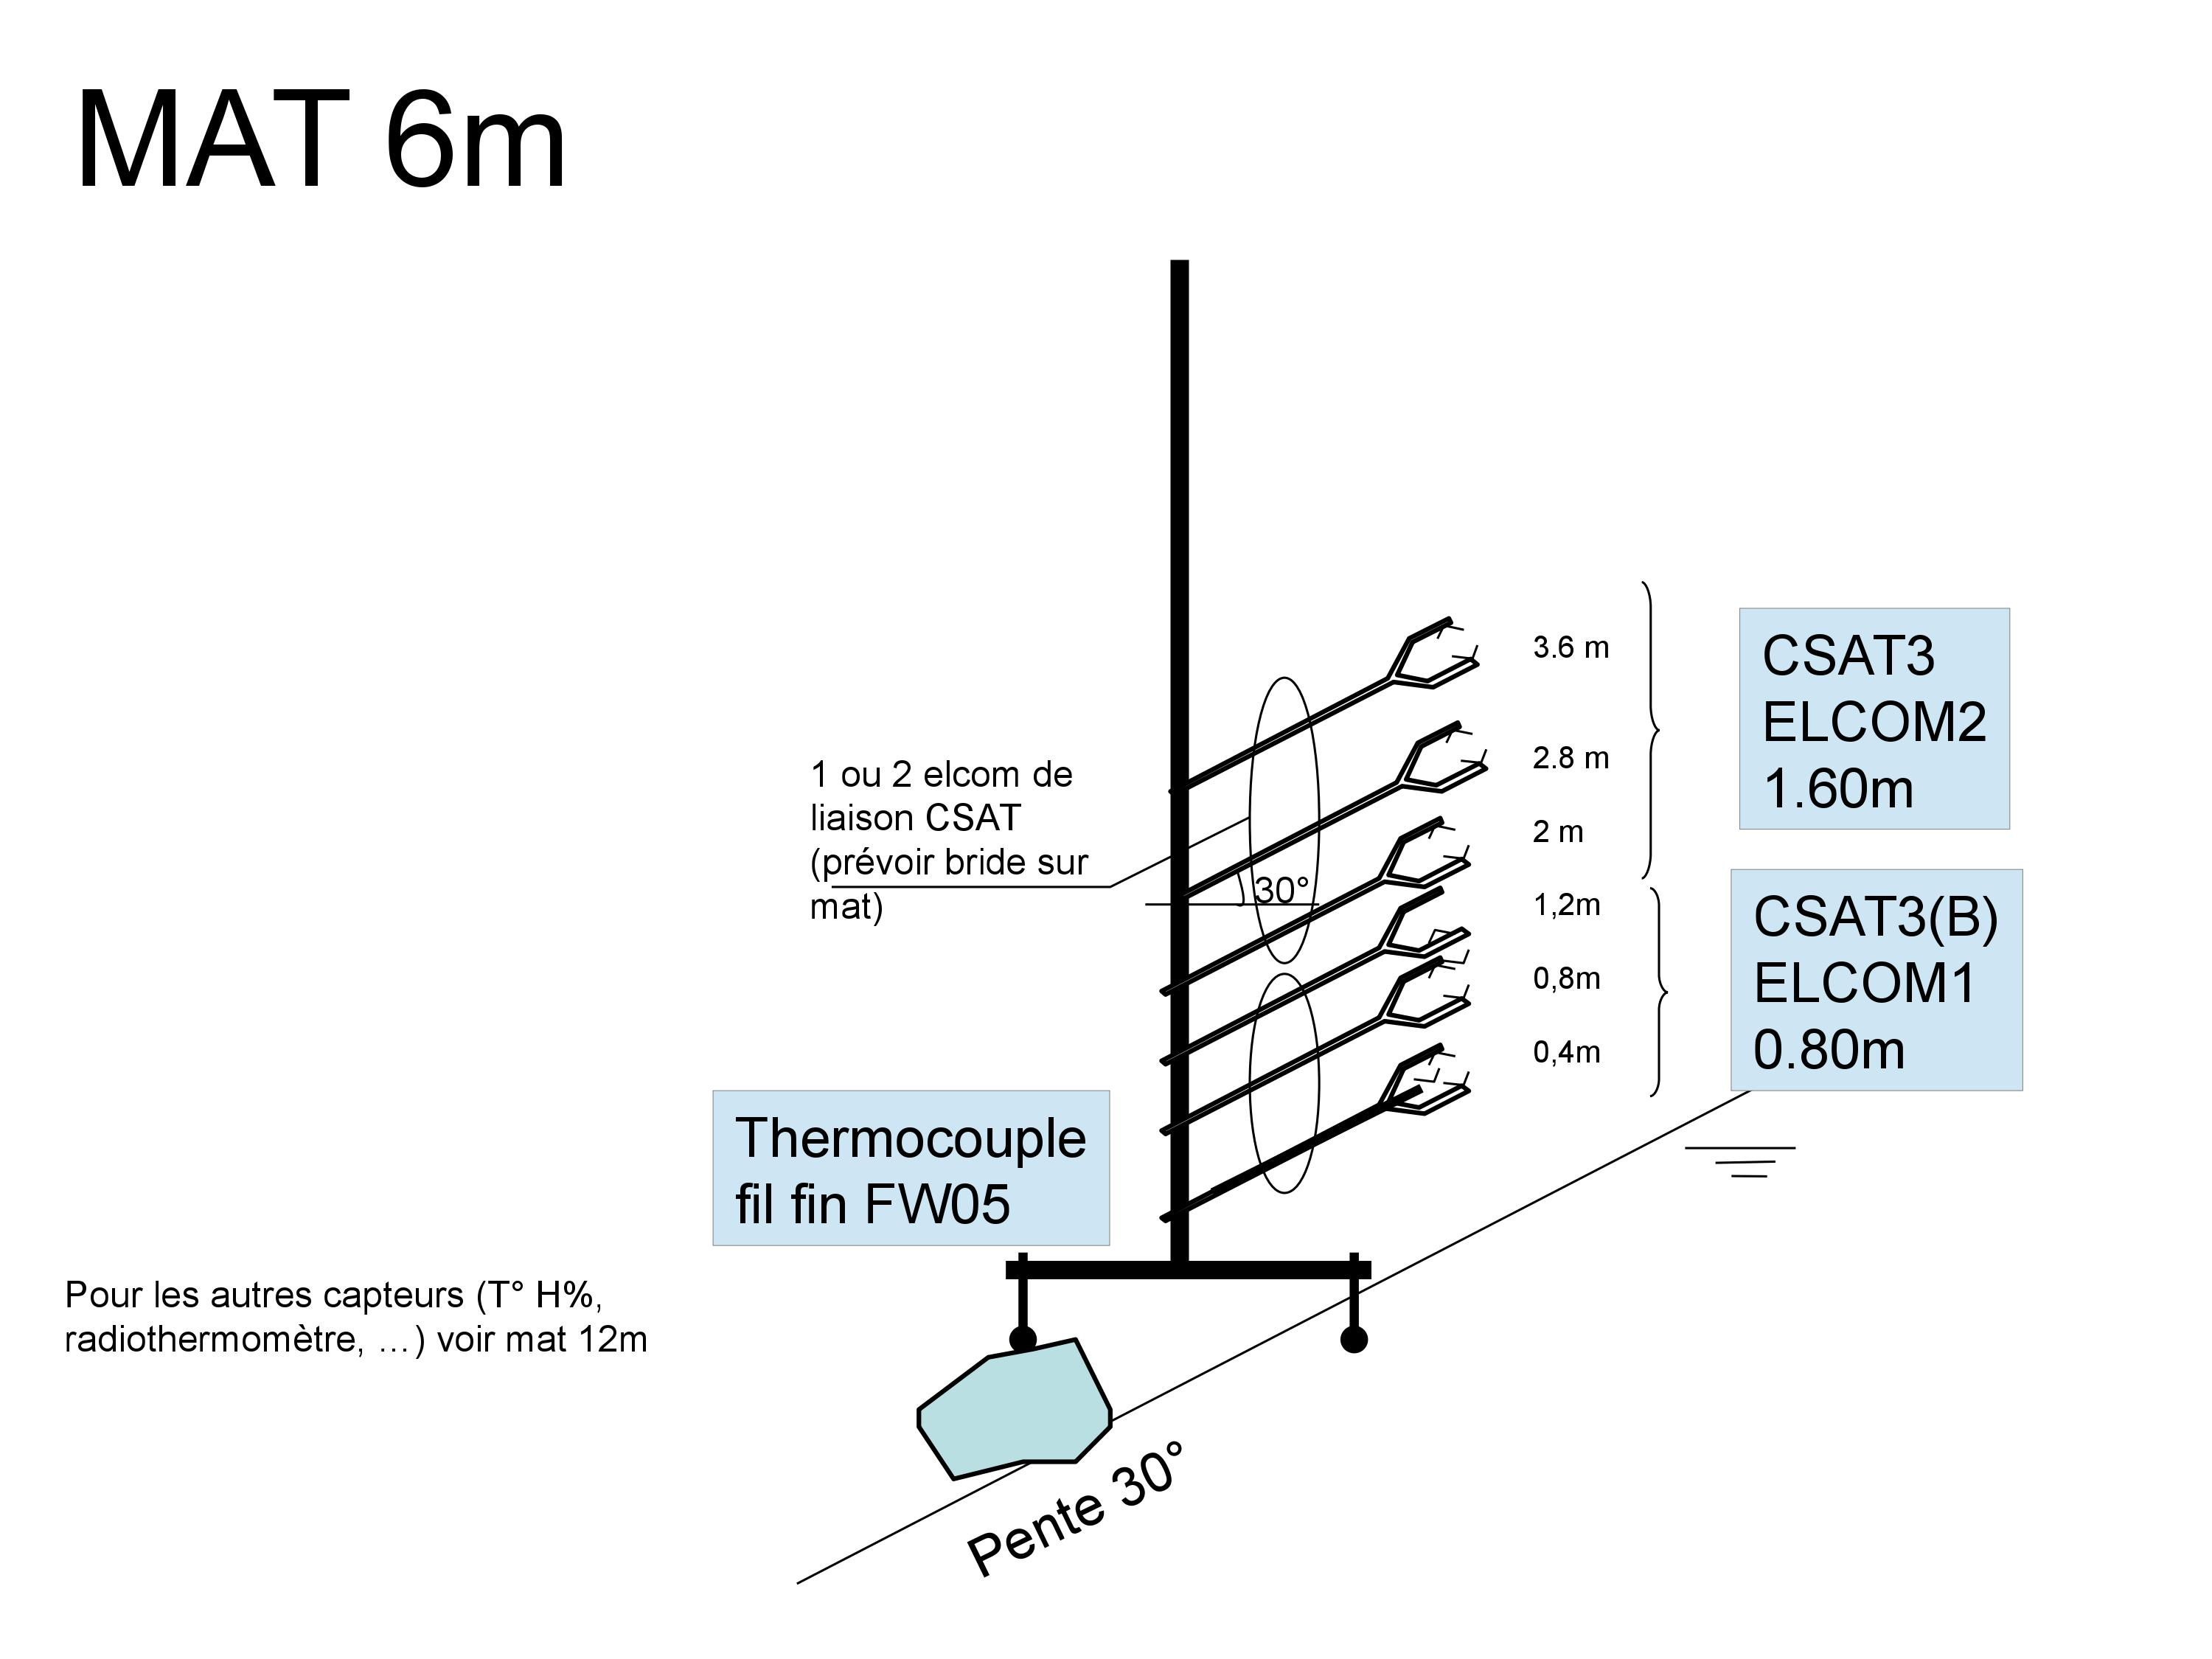
\includegraphics[width=0.7\textwidth]{fig/0001.jpg}
  \caption{Placement of the instruments on the 6~m mast. Along the mast, there are six CSAT3 Sonic Anemometers.}
  \label{fig:mast_6}
  \end{center}
\end{figure}

In figure~\ref{fig:mast_12} we see the mast that is 12~m high. At the top we can see a Windmaster 3D ultrasonic anemometer, that can measure the three components of wind with a frequency up to 20~Hz. Bellow it, we can see three Gill Windmaster anemometers, that are located between 9.5~m and 5.5~m. And at 4.2~m, there is a Vaisala 2D anemometer.  All the anemometers measure the direction and speed of wind with a frequency that depends on the model of the sensor. 

Spread along the mast, there are nine thin film thermocouples, that are used to measure the temperature of air with minimal intrusion. In the middle, there is a radiometer used to measure the radiant flux. Finally, there is an ultrasonic instrument installed in the station (not shown in the figures) to record the height of the snow cover. Snow-covered ground is expected in the measuring site. This is important because the snow diminishes the roughness of the ground.

\begin{figure}[!ht]
  \begin{center}
  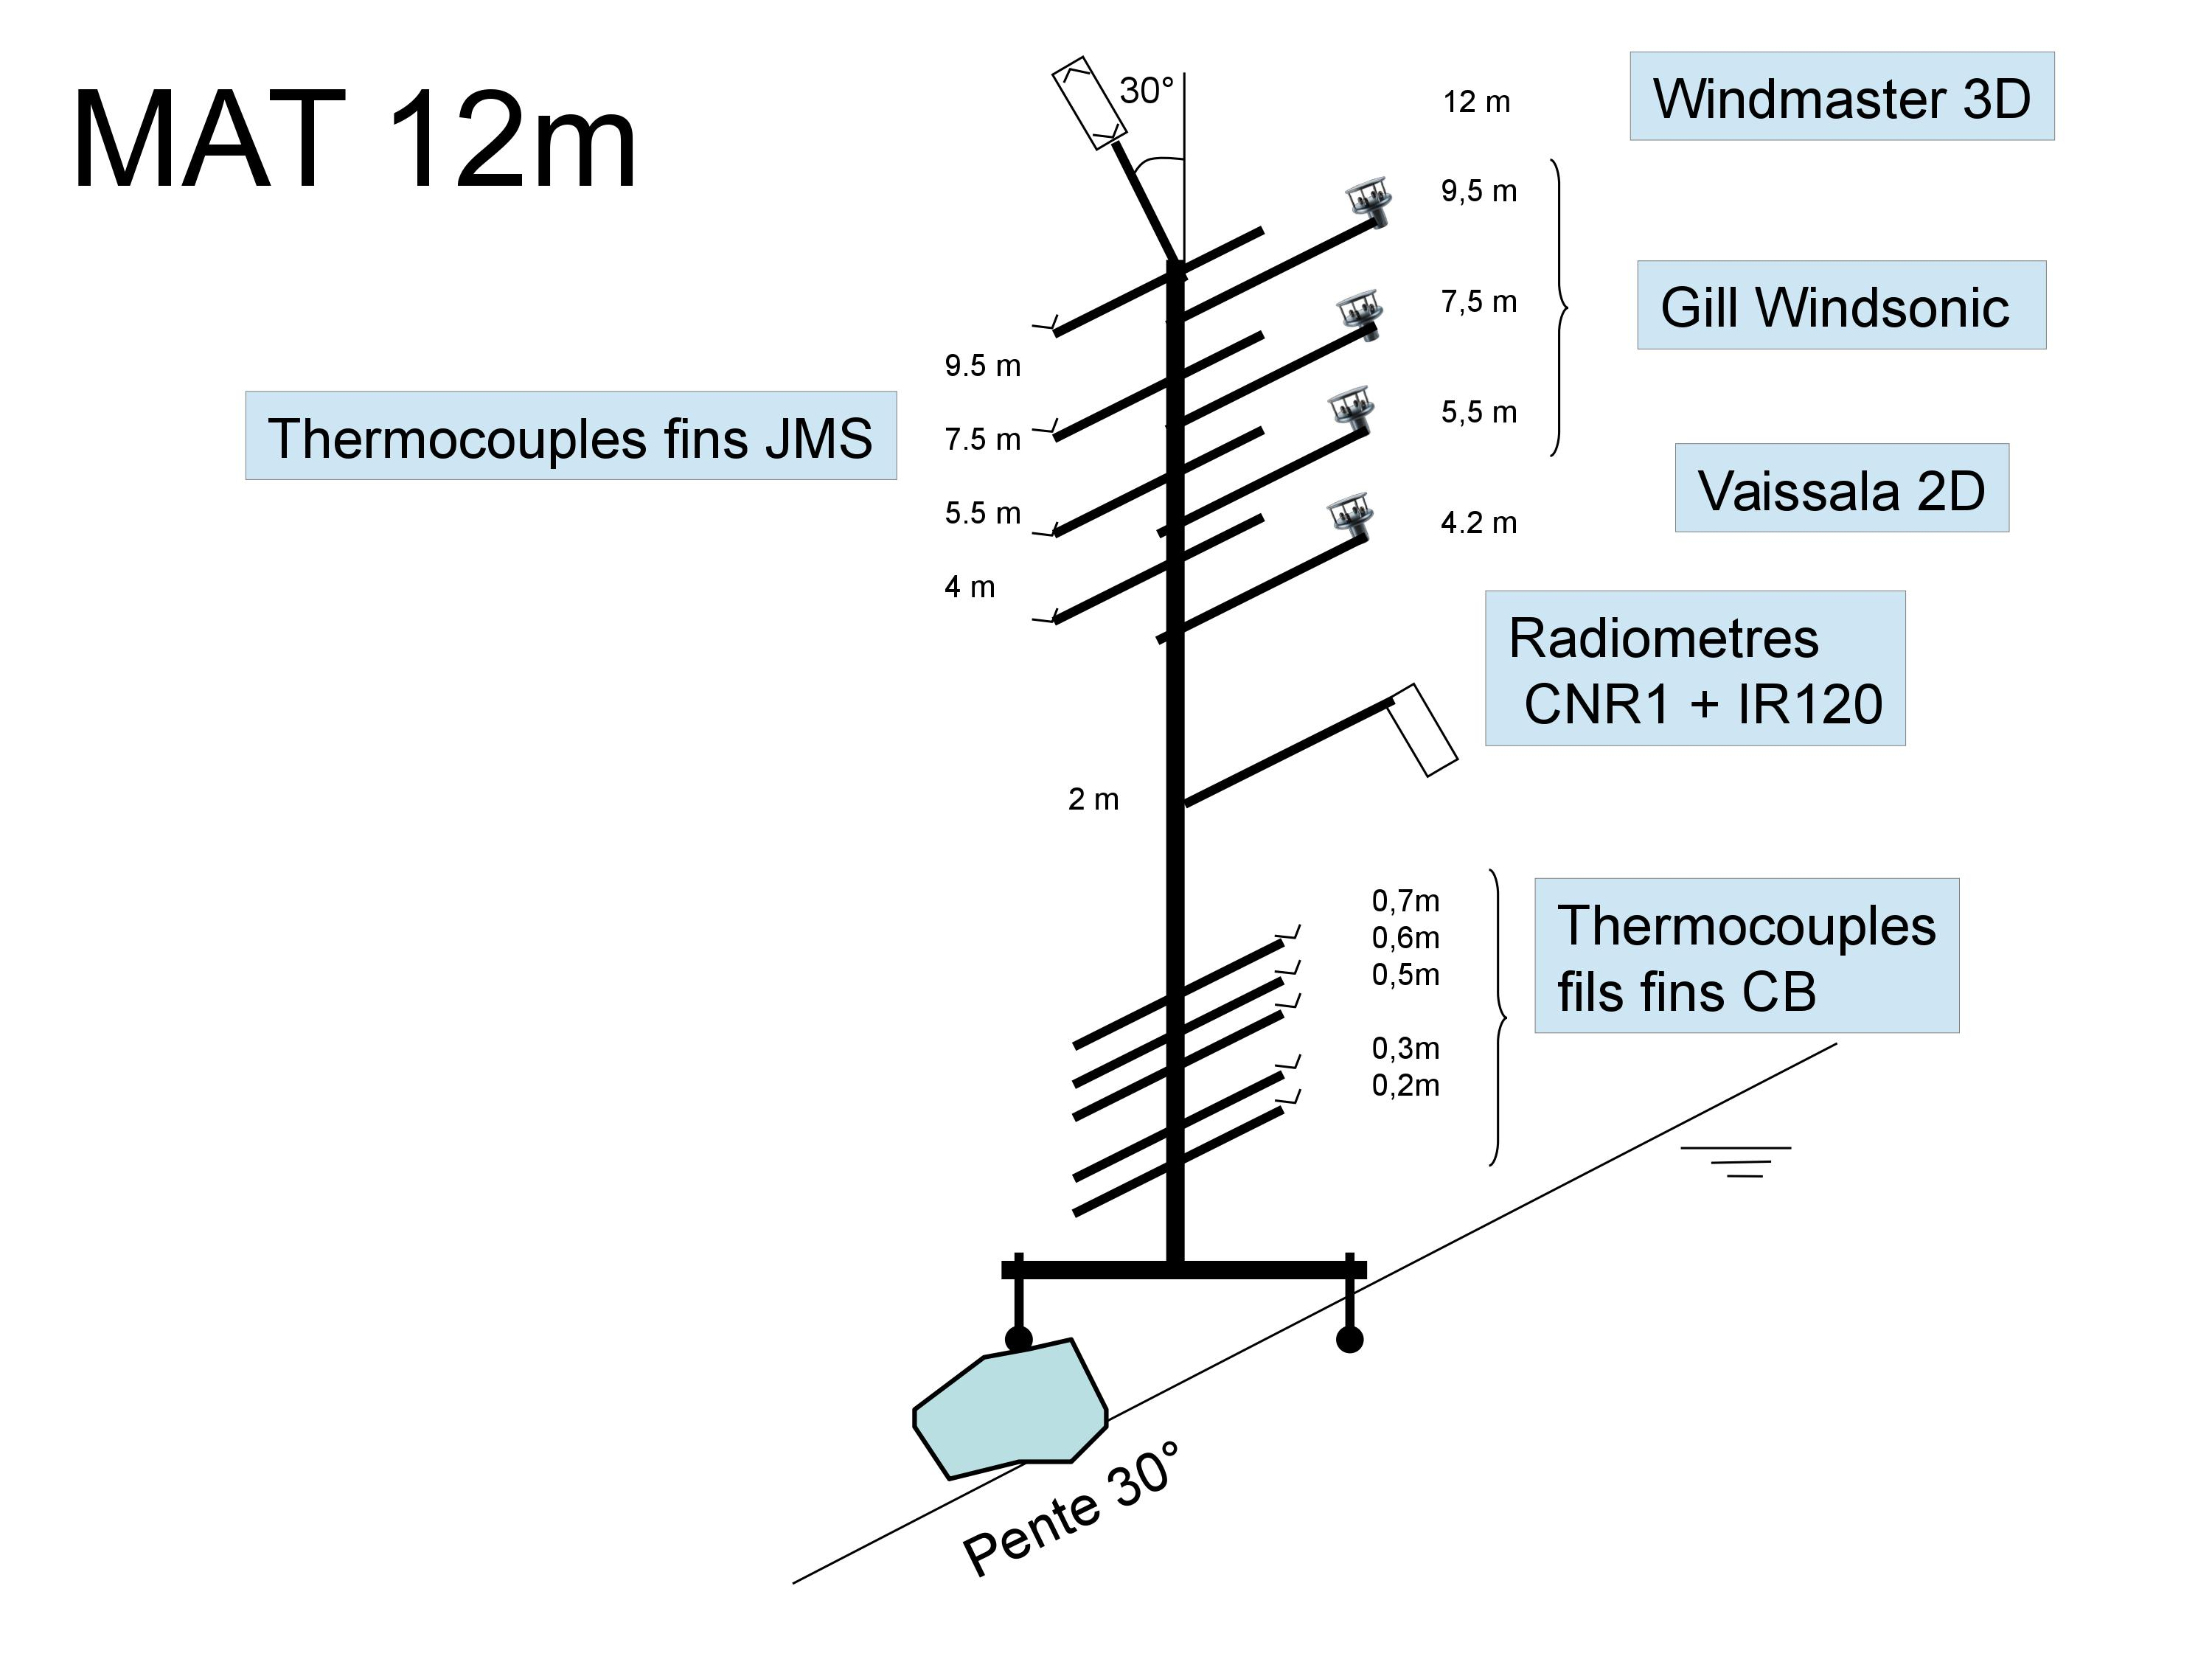
\includegraphics[width=0.7\textwidth]{fig/0002.jpg}
  \caption{Placement of the instruments on the 12~m mast.}
  \label{fig:mast_12}
  \end{center}
\end{figure}

\section{Timetable}
The timetable~\ref{table:schedule} shows the planning for the activities to do during the next five months. 

\begin{table}[ht!]
%\centering
\begin{center}
\begin{tabular}{|c|c|p{9.5cm}|}
\hline
  & \textbf{Working days} & \textbf{Activity} \\
\hline
January & 1 & Field Work\footnote{\label{note1}The date of the field campaign is not set. It must occur during winter (January and February), when there are anticyclonic conditions.}. Working on theory and foundations of the research.\\
\hline
February & 7 & Field Work$^2$. Analysis of the data, start to analyse 2015 data to get familiar with EddyPro.\\
\hline
March & 4 & Analysis of the data gathered during the field work.\\
\hline
April & 7 & Writing and analysing the data gathered.\\
\hline
May & 12 & Plotting the results and final analysis of the data sets. Working in the final report and oral presentation.\\
\hline
\end{tabular}
\caption{Research project schedule showing the number of working days per month and the tasks to work on.}
\label{table:schedule}
\end{center}
\end{table}



\clearpage
%\medskip
%\nocite{*}
\bibliographystyle{plainnat}
\bibliography{biblio}
%\printbibliography

\end{document}
